% The nested squares of a spot code, with the characters of the compound Hafia 3 · 1230: 0 22JV PVQQ.
\documentclass[border=2mm]{standalone}
\usepackage{fontspec}\setmainfont{LibertinusSans}[Extension=.otf,UprightFont=*-Regular,BoldFont=*-Bold]
\usepackage{unicode-math}\setmathfont{LibertinusMath-Regular.otf}
\setmonofont{LibertinusMono-Regular.otf}
\usepackage{tikz}
\definecolor{ink}{HTML}{0B5C35}\definecolor{hit}{HTML}{2A78D6}
\providecommand{\T}[2]{#1}% \T{English}{French}; the -fr wrappers select the French text
\begin{document}
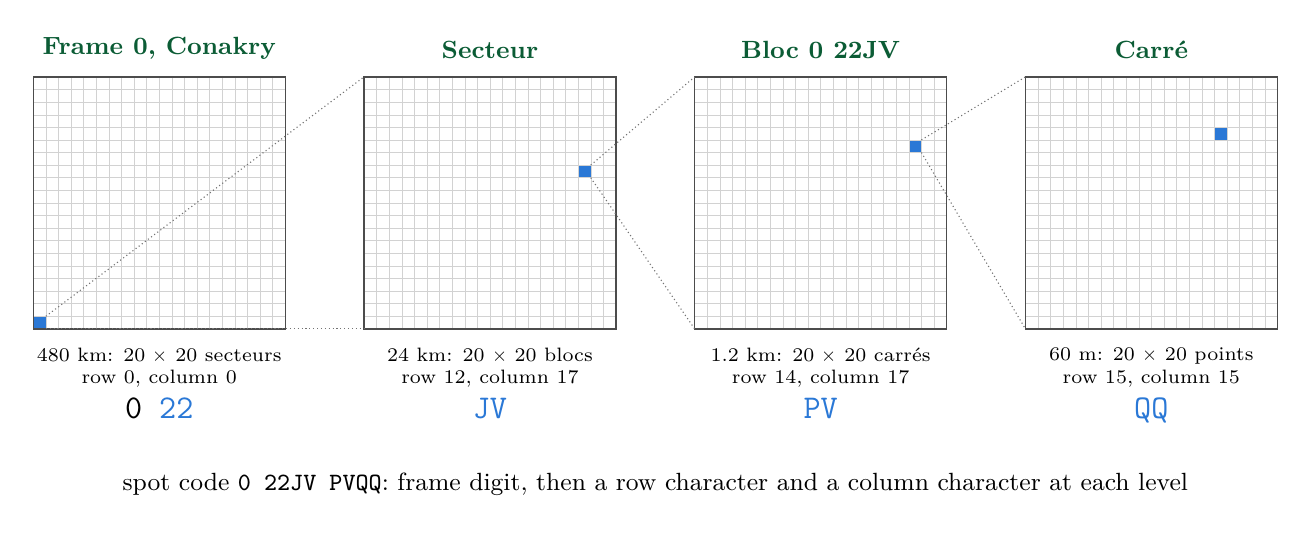
\begin{tikzpicture}[x=1mm, y=1mm]
% each panel: 20 x 20 squares of 1.6 mm; (r, c) counted from the south-west corner
\newcommand{\panel}[6]{% x0, row, col, title, side, chars
  \begin{scope}[shift={(#1,0)}]
    \fill[hit] (#3*1.6, #2*1.6) rectangle ++(1.6,1.6);
    \draw[gray!35, line width=0.15pt] (0,0) grid[step=1.6] (32,32);
    \draw[black!70, line width=0.5pt] (0,0) rectangle (32,32);
    \node[anchor=south, font=\small\bfseries, text=ink] at (16,33) {#4};
    \node[anchor=north, font=\scriptsize, align=center] at (16,-1.2) {#5};
    \node[anchor=north, font=\ttfamily\large] at (16,-7.5) {#6};
  \end{scope}}
\panel{0}{0}{0}{\T{Frame 0, Conakry}{Cadre 0, Conakry}}{480 km\T{:}{ :} 20 $\times$ 20 secteurs\\\T{row 0, column 0}{rangée 0, colonne 0}}{0 \textcolor{hit}{22}}
\panel{42}{12}{17}{Secteur}{24 km\T{:}{ :} 20 $\times$ 20 blocs\\\T{row 12, column 17}{rangée 12, colonne 17}}{\textcolor{hit}{JV}}
\panel{84}{14}{17}{Bloc 0 22JV}{\T{1.2}{1,2} km\T{:}{ :} 20 $\times$ 20 carrés\\\T{row 14, column 17}{rangée 14, colonne 17}}{\textcolor{hit}{PV}}
\panel{126}{15}{15}{Carré}{60 m\T{:}{ :} 20 $\times$ 20 points\\\T{row 15, column 15}{rangée 15, colonne 15}}{\textcolor{hit}{QQ}}
\foreach \a/\b/\r/\c in {0/42/0/0, 42/84/12/17, 84/126/14/17}{
  \draw[black!55, line width=0.4pt, densely dotted] (\a+\c*1.6+1.6, \r*1.6+1.6) -- (\b, 32);
  \draw[black!55, line width=0.4pt, densely dotted] (\a+\c*1.6+1.6, \r*1.6) -- (\b, 0);
}
\node[anchor=north, font=\small] at (79,-17) {\T{spot code \texttt{0 22JV PVQQ}: frame digit, then a row character and a column character at each level}{code de point \texttt{0 22JV PVQQ} : chiffre du cadre, puis un caractère de rangée et un caractère de colonne à chaque niveau}};
\end{tikzpicture}
\end{document}
